\documentclass[a4paper,12pt,bibliography=totocnumbered]{scrartcl}

\usepackage[utf8]{inputenc} 
\usepackage[T1]{fontenc}
\usepackage[ngerman]{babel} 
\usepackage{amsmath, amssymb,amsfonts}
\usepackage{graphicx}
\usepackage{csquotes}
\usepackage[bookmarks,colorlinks=true]{hyperref}
\usepackage{geometry}
\usepackage{float}
\usepackage[final]{pdfpages}
\usepackage{framed, color} 
\usepackage{scrlayer-scrpage}
\usepackage{siunitx}
\usepackage{subfigure}
\renewcaptionname{ngerman}{\figurename}{Abb.}
\sisetup{detect-weight=true, detect-family=true,locale=DE,range-phrase={\,bis\,},list-final-separator ={\,\linebreak[0] \text{und}\,},separate-uncertainty=true,per-mode = symbol-or-fraction}
\DeclareSIUnit\curie{Ci}
\usepackage[backend=biber, style=chem-angew]{biblatex} 
\addbibresource{lit.bib} 

\usepackage{chemgreek}
\usepackage{chemformula}
\geometry{left = 2.5cm} \geometry{top= 3cm}

\urlstyle{same}
%Hyperlinks-Setup
\hypersetup{
	colorlinks,
	linktocpage,
	citecolor=black,
	filecolor=black,
	linkcolor=black,
	urlcolor=black
}

%\numberwithin{equation}{section}

\setlength{\parindent}{0 mm}
\setlength{\parskip}{2 mm} 



\pagestyle{scrheadings}
%Header oben links auf linker Seite (ungerade Seitenzahl) und oben rechts auf rechter Seite (gerade Seitenzahl), beinhaltet gruppennummer und Versuchskürzel. Im Fall eine einseitigen Dokuments: Header oben rechts
\ihead{\VerfasserEINS\;\&\;\VerfasserZWEI} %Header oben rechts auf linker Seite und oben links auf rechter Seite. Beinhaltet die Namen der Verfasser. Im Fall eine einseitigen Dokuments: Header oben links!
\ofoot{\thepage} %Footer unten links auf linker und unten rechts auf rechter Seite, enthält die jeweilige Seitenzahl. Im Fall eines einseitigen Elements: Footer unten rechts!
\cfoot{\empty} %Mittig unten im Footer soll nichts eingetragen werden 
\ifoot{\empty} %Footer unten rechts auf linker und unten links auf rechter Seite. Hier ebenfalls leer.


\newcommand{\VERSUCHSDATUM}{20.10.-28.10.2025}
\newcommand{\PROTOKOLLDATUM}{\today}

\newcommand{\VerfasserEINS}{Vincent Kümmerle}
\newcommand{\MatNoEINS}{3712667}
\newcommand{\EmailEINS}{st187541@stud.uni-stuttgart.de}
\newcommand{\StudiengangEINS}{B.Sc. Chemie}

\newcommand{\VerfasserZWEI}{Elvis Gnaglo}
\newcommand{\MatNoZWEI}{3710504}
\newcommand{\EmailZWEI}{st189318@stud.uni-stuttgart.de}
\newcommand{\StudiengangZWEI}{B.Sc. Chemie}

\newcommand{\BETREUER}{Benjamin Knies}
\newcommand{\GRUPPENNR}{A05}

\newcommand{\VERSUCHSNR}{Festkörper Präparat}
\newcommand{\VERSUCHSNAME}{Cobalteisenstein}


\begin{document}
\thispagestyle{empty}


\begin{titlepage}

\begin{center}
\Huge{\textbf{\VERSUCHSNR\ - \VERSUCHSNAME}}\\
\vspace{10mm}% Abstand
\Large{Protokoll zum Versuch des AC2 Praktikums von \\ \textbf{\VerfasserEINS\;\& \VerfasserZWEI}}\\
\vspace{10mm} 
\Large{Universität Stuttgart}\\
\end{center}
\vspace{1cm}
\begin{center}
\begin{tabular}{ll}
\large{Verfasser:}		& \large{\VerfasserEINS,} \large{\MatNoEINS} \\
 						& \large{\EmailEINS} \\
 						\vspace{0cm}\\
						& \large{\VerfasserZWEI,} \large{\MatNoZWEI} \\
                        & \large{\EmailZWEI} \\
						\vspace{0cm}\\
\large{Gruppennummer:}	& \large{\GRUPPENNR} \\
\vspace{0cm}\\
\large{Versuchszeitraum:}	& \large{\VERSUCHSDATUM} \\
\vspace{0cm}\\
\large{Betreuer:}		& \large{\BETREUER} \\
\vspace{0cm}\\
\large{Abgabenummer:} & \large{1. Abgabe}
\end{tabular}
\end{center}
\vspace{15mm}

\begin{center}
Stuttgart, den \PROTOKOLLDATUM
\end{center}

\end{titlepage}


\thispagestyle{empty}

\tableofcontents 

\clearpage

\renewcommand{\thepage}{\arabic{page}}
\setcounter{page}{1}


\section{Einleitung}
Cobalteisenstein weckte bereits in den frühen 1930er Jahren in Japan großes Interesse. 
Besonders fiel es durch seinen hohen elektrischen Widerstand, die hohe Remanenz und Koerzitivkraft auf, bevor es als nichtleitender Permanentmagnet ab Anfang 1950 durch das günstiger herzustellende Bariumferrit abgelöst wurde.
\cite{History}.
Heutzutage finden Cobaltferritnanopartikel Verwendung für Magnetspeichersysteme mit hoher Kapazität und als Katalysator für die Oxidation von Alkenen. \cite{Rieck},\cite{Kat} \\
Das Ziel des Versuchs war die Synthese und Charakterisierung der Struktur von \ch{CoFe2O4} mit Röntgen-Pulverdiffraktometrie.

\section{Struktur}
Cobalteisenstein kristallisiert in der Spinellstruktur. \cite{Rieck} 
%und weist die Raumgruppe $Fd \overline{3} m$ auf. 
Im Zuge der Strukturbeschreibung stellt sich die Frage nach der Kationenverteilung. 
Dazu wird die Ligandenfeldaufspaltungsstabilisierungsenergie (LSFE) im inversen Spinell mit \ch{Co^{2+}} in den Oktaederlücken im Vergleich zum normalen Spinell mit \ch{Co^{2+}} in den Tetraederlücken berechnet. 
Da die LSFE im inversen Spinell höher ist, ergibt sich für den inversen Spinell eine günstigere Stabilisierung.
Die in \autoref{fig: Elementarzelle} dargestellte Elementarzelle des Cobalteisensteins besteht aus einer kubisch-dichtesten Kugelpackung der \ch{O^{2-}}-Anionen, wobei $\frac{1}{8}$ der Tetraederlücken mit \ch{Fe^{3+}}, 
$\frac{1}{4}$ der Oktaederlücken mit \ch{Fe^{3+}} und $\frac{1}{4}$ der Oktaederlücken mit \ch{Co^{2+}} besetzt sind. \\

\begin{figure}[H]
    \centering
    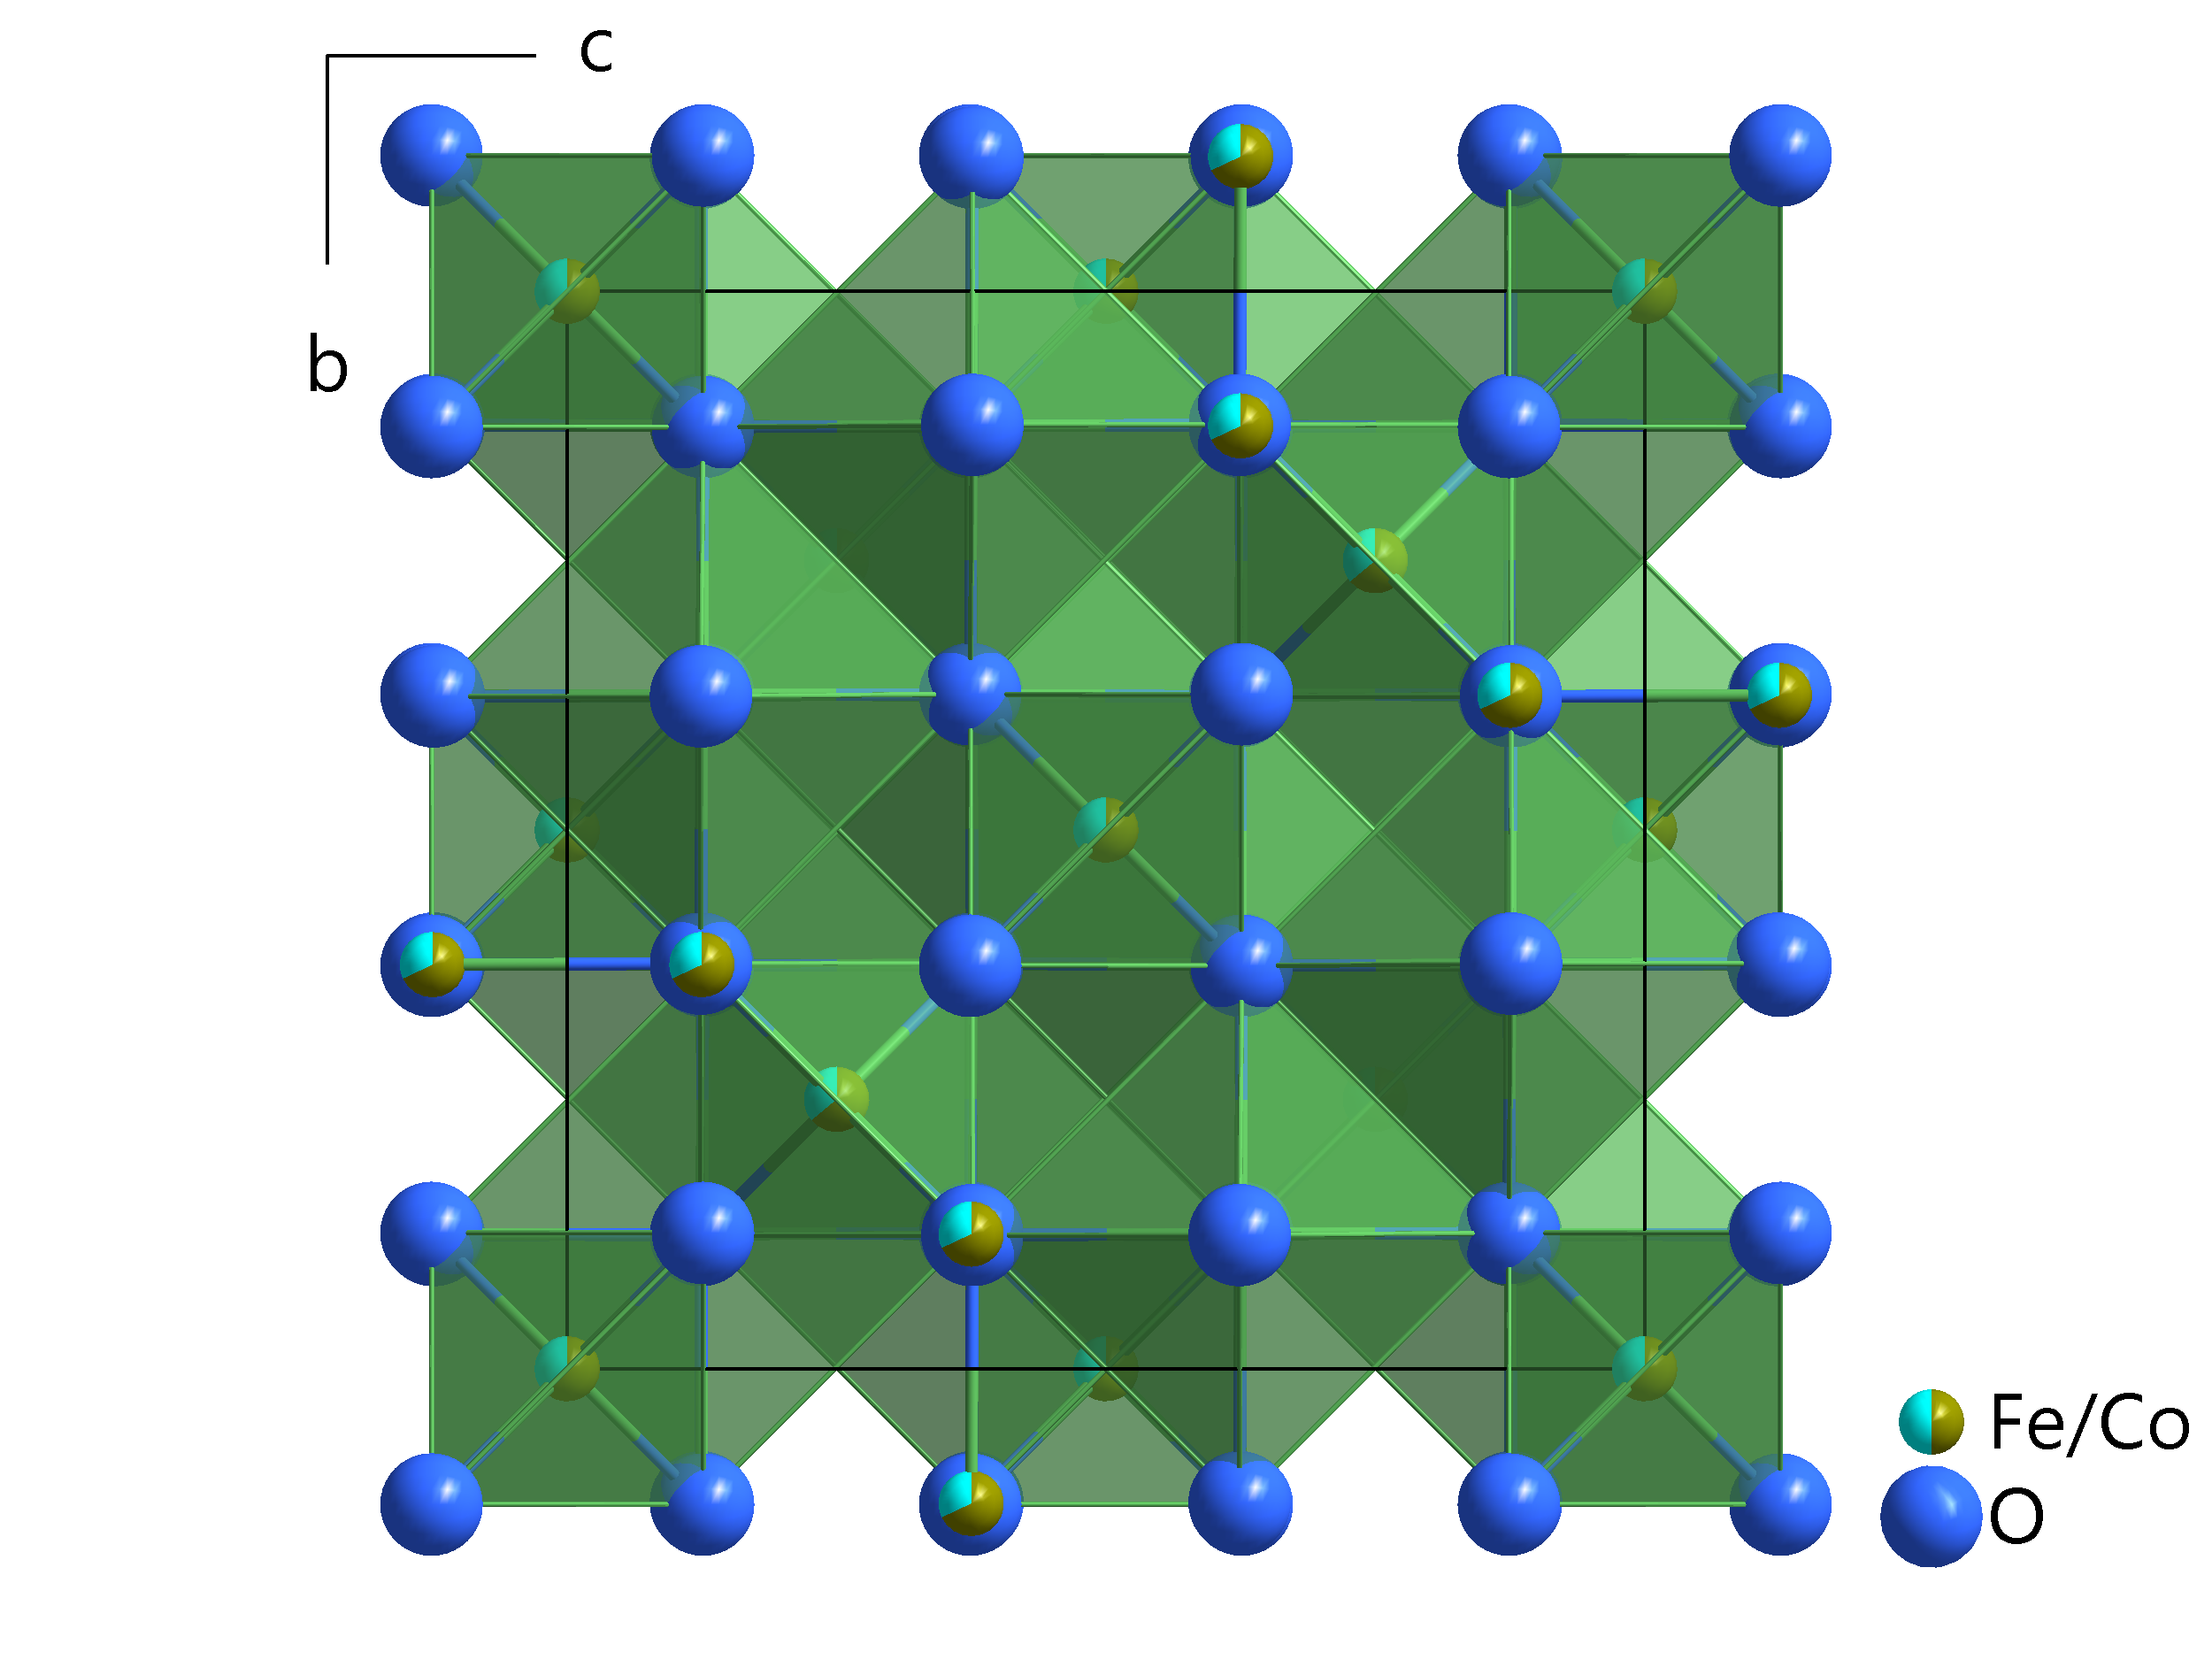
\includegraphics[width=0.75 \linewidth ]{Bilder/Elementarzelle.png}
    \caption{Elementarzelle des \ch{CoFe2O4}.\cite{Rieck}}
    \label{fig: Elementarzelle}
\end{figure}

Tatsächlich sind die Kationen jedoch zufällig auf die Tetraeder- und Oktaederlücken verteilt \cite{Rieck}.
Dies lässt sich darauf zurückführen, dass \ch{Co^{2+}} einen kleineren Ionenradius als \ch{Fe^{3+}} aufweist und somit auch die Tetraederlücken besetzt, da diese eine geringere Bindungslänge zwischen Zentralkation und den \ch{O^{2-}}-Anionen als die Oktaederlücken aufweist.
Dies ist im Strukturausschnitt in \autoref{fig: TL} aufgezeigt, in dem vier Anionen tetraedrisch um ein Metallkation angeordnet sind, wohingegen es in der Oktaederlücke in \autoref{fig: OL} sechs Anionen sind.


\begin{figure}[H]
    \centering
    \includegraphics[scale=0.1]{Bilder/Tetraederlücke.png}
    \caption{Tetraederlücken in \ch{CoFe2O4}.\cite{Rieck}}
    \label{fig: TL}
\end{figure}

\begin{figure}[H]
    \centering
    \includegraphics[scale=0.15]{Bilder/Oktaederlücke.png}
    \caption{Oktaederlücken in \ch{CoFe2O4}.\cite{Rieck}}
    \label{fig: OL}
\end{figure}

% Magnetismus von Cobalteisenstein
Die magnetischen Eigenschaften von Cobalteisenstein sind auf die Kopplung der magnetischen Momente der ungepaarten d-Elektronen der Metallionen in  der inversen Spinellstruktur zurückzuführen. \cite{Müller}
Die indirekten Superaustausch-Wechselwirkungen über die Oxidanionen führt dazu, dass sich die Spins der Metallionen in den Tetraeder- und Oktaederlücken antiparallel zueinander ausrichten, wobei sehr viele dieser Gitterlücken eine magnetische Domäne bilden. \\
Wenn ein äußeres Magnetfeld angelegt wird, steigt die Anzahl der Domänen mit Magnetisierung in Feldrichtung, während die Anzahl der Domänen mit der entgegengesetzten Ausrichtung sinkt. 
Diese Eigenschaft verschieden großer magnetischer Momente ist charakteristisch für ferrimagnetische Substanzen, da sich so die magnetischen Momente auch bei tiefen Temperaturen nicht kompensieren. 
Dadurch verhält sich Cobalteisenstein im Magnetfeld wie ein Ferromagnet, obwohl die mikroskopische Ordnung antiparallel ist. \cite{Müller}

\section{Charakterisierungsmethoden}

\subsection{Erzeugung von Röntgenstrahlung}
Die hergestellte Verbindung wird mit Hilfe der Pulverdiffraktometrie charakterisiert.
Dabei zeigt \autoref{fig: Röhre}, wie Elektronen über eine Heizspannung aus einer Wolframkathode in das Vakuum der Röntgenröhre geleitet und über die dort angelegte Spannung zur Kupferanode beschleunigt werden.
An der Anode können die freien Elektronen auf Elektronen in den inneren Schalen treffen und diese ``herausschlagen``. \cite{Kristallgitter}
%Bild RÖhre
\begin{figure}[H]
    \centering
    \includegraphics[scale=0.3]{Bilder/RÖhre.jpg}
    \caption{Aufbau der Röntgenröhre mit Wasserkühlung, W-Kathode, Cu-Anode und Be-Fenster. \cite{Kristallgitter}}
    \label{fig: Röhre}
\end{figure}
Der dadurch erzeugte Elektronenmangel in der Schale wird durch ein Elektron aus einer höheren Schale ausgeglichen, wobei dieses beim Wechseln der Schalen Energie in Form von charakteristischer Röntgenstrahlung freisetzt. 
Einige Elektronen dringen stattdessen bis zum Atomkern vor. 
Dort werden sie durch Wechselwirkungen mit dem Kern unter Abgabe von Röntgenstrahlung als Bremsstrahlung mit vielen verschiedenen Wellenlängen abgelenkt.
Beide Arten von Strahlung treten durch ein Berylliumfenster aus der andernfalls abgeschirmten Apparatur aus. 
\newpage
Da diese Strahlung somit für eine Analyse nicht präzise genug ist, wird die austretende Strahlung durch einen Monochromator wie Ni-Folie und einen Kollimator geleitet, wodurch nur die Strahlung der charakteristischen Wellenlänge des Übergangs auf die Probe trifft. 
Durch Ablenkung der Röntgenstrahlung am Kristallgitter der Probe können Beugungsreflexe detektiert werden, die durch ihre Intensität und räumliche Anordnung auf die Geometrie des Kristallgitters schließen lassen.

\subsection{Röntgenbeugung}
% Warum Röntgenstrahlung?
Diese Analysemethode verwendet spezifisch Röntgenstrahlung, da sich die Wellenlänge der Strahlung in der gleichen Größenordnung wie die Gitterkonstante befindet. \cite{Kristallgitter}
Dadurch lässt sich auch erklären, wie die Strahlung am Kristallgitter der Verbindung gebeugt werden kann.
Es ist essenziell, dass die Wellenlänge nicht zu klein ist, um ungehindert durch das Gitter zu kommen, da so keine Beobachtungen möglich wären.
Allerdings darf die Wellenlänge aber auch nicht zu groß sein, da die Reflexe so verbreitert und damit unscharf werden würden.
% Ort der Beugung

% Interferenz am Gitter
Wird ein Kristallgitter mit monochromatischem Licht bestrahlt, so tritt bei positiver Überlagerung der kugelförmigen Streuwellen konstruktive Interferenz auf, wenn der Gangunterschied $\Delta$ zwischen benachbarten Wellen ein Vielfaches von $\lambda$ beträgt. \cite{Kristallgitter}
Deswegen lassen sich nur an diesen ``erlaubten`` Stellen, an denen die Interferenzbedingung für alle Gitterpunkte gilt, im Raum scharfe Reflexe beobachten.

% Netzebenen (Beschreibung, Benennung)
Die durch drei Punkte des Translationsgitters festgelegten Ebenen, an denen die Reflexion stattfindet, werden Netzebenen genannt. 
Zur Charakterisierung von Netzebenen werden die Miller-Indices $hkl$ genutzt. Sie geben die Kehrwerte der Achsenabschnitte $\frac{1}{h}$, $\frac{1}{k}$ und $\frac{1}{l}$ von der Ebene, die dem Nullpunkt am nächsten liegt, mit der a-,b- und c-Achse der Elementarzelle an. 
Dabei geht die Ebene nicht durch den Nullpunkt hindurch und die Indices der Flächen ($hkl$) sind ganze Zahlen, die angeben, wie oft eine Achse durch eine Netzebenenschar untergliedert wird. 
Für die davon ausgehenden Reflexe werden die Miller-Indices ohne Klammern verwendet. \\
Aus der Spiegelbedingung für eine Netzebene bei konstruktiver Interferenz geht hervor, dass beim Strahlengang (siehe \autoref{fig: Bragg}) der Einfallswinkel $\theta$ gleich dem Ausfallswinkel sein und zusätzlich einen speziellen Wert aufweisen muss, bei dem alle Streuwellen im ganzen Translationsgitter in Phase sind. 
Dieser Winkel lässt sich aus dem Gangunterschied $2 \cdot d \cdot \sin \theta$ einer Welle, die an der nächst tiefer im Gitter liegenden Ebene reflektiert wird, mit der Bragg-Gleichung (siehe \autoref{Bragg}) bestimmen. 
\begin{equation}
    2 \cdot d \cdot \sin \theta = n \cdot \lambda
    \label{Bragg}
\end{equation}

\begin{figure}[H]
    \centering
    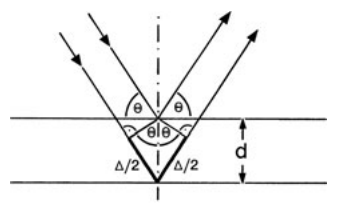
\includegraphics[scale=0.95]{Bilder/Bragg.png}
    \caption{Strahlengang des gebeugten Strahls nach Auftreffen auf das Gitter. \cite{Kristallgitter}}
    \label{fig: Bragg}
\end{figure}
Somit muss der Gangunterschied mit dem Netzebenenabstand $d$ einem  ganzzahligen Vielfachen der Wellenlänge $\lambda$ entsprechen, damit die betrachteten Einfallswinkel $\theta$ erlaubt sind.
Damit sind die möglichen Winkel für verschiedene Beugungsordnungen $n$ festgelegt.
%Der Beugungswinkel $2\theta$ zwischen einfallendem und ausfallendem Strahl lässt sich experimentell bestimmen lässt.


\section{Durchführung}
Es wurden 1 Äquivalent \ch{Co3O4}(85 mg; 0,352 mmol) und 3 Äquivalente \ch{Fe2O3}(170 mg; 1,066 mmol) abgewogen und im Mörser zu einem feinen Pulver zerkleinert. 
Anschließend wurde das Gemisch in einen Porzellantiegel überführt und für 48 Stunden bei $800 ^\circ$C im Ofen erhitzt.\\
Nach Abkühlen an der Luft wurde ein dunkelgraues Pulver erhalten. 
Dieses wurde anschließend erneut mit dem Mörser zu einem feinen Pulver gemahlen und auf den Probenträger des Pulverdiffraktometers getragen. 
Der Probenträger wurde danach in das Pulverdiffraktometer gespannt und die Probe wurde für 20 Minuten durch kontinuierliche Drehung und Bestrahlung mit Cu-K$_\alpha$-Strahlung analysiert.

\newpage

\section{Ergebnisse}
Die \autoref{fig: prettyplot} zeigt das gemessene Diffraktogramm der hergestellten Verbindung und 
die aus Einkristalldaten simulierten Diffraktogramme von Cobalteisenstein und Eisen(III)oxid, 
wobei die relative Intensität gegen den Beugungswinkel $\theta$ aufgetragen wurde. 
\begin{figure}[H]
    \centering
    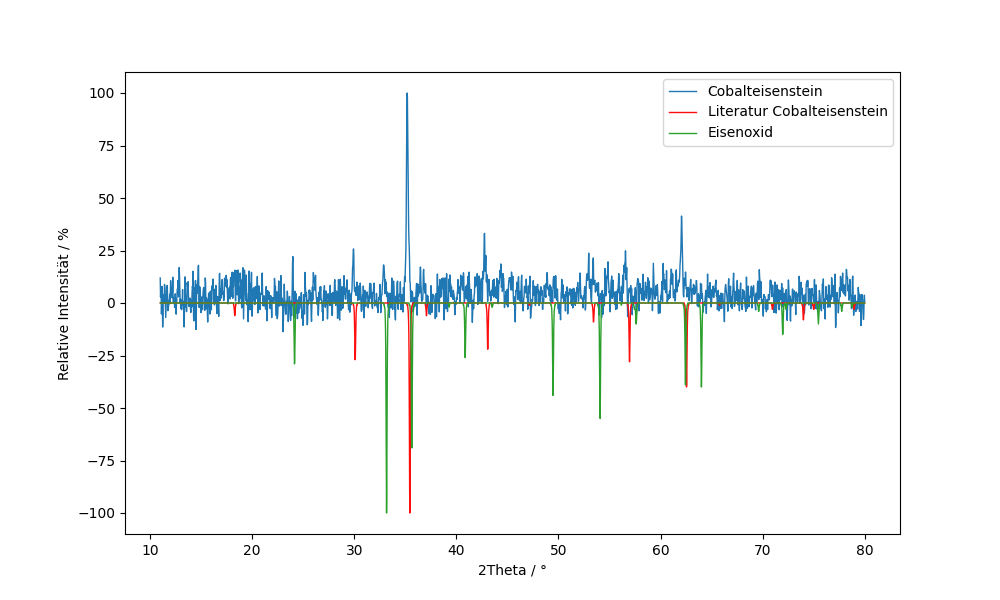
\includegraphics[scale=0.65]{Bilder/messreihen.png}
    \caption{Diffraktogramm des hergestellten \ch{CoFe2O4} (Blau) im Vergleich mit den aus Einkristalldaten simulierten Diffraktogrammen von \ch{CoFe2O4} (Rot) und \ch{Fe2O3} (Grün). \cite{Rieck},\cite{FeDiff}}
    \label{fig: prettyplot}
\end{figure}

Das Diffraktogramm zeigt, dass die Intensitätsmaxima der hergestellten Verbindung im Großteil mit denen der Simulation von Cobalteisenstein übereinstimmt.
Dadurch wurde bewiesen, dass Cobalteisenstein hergestellt wurde. Es sind allerdings noch weitere Intensitätsmaxima beobachtbar, die mit denen aus der Simulation von Eisen(III)oxid übereinstimmen.
Dies macht erkenntlich, dass Spuren von Eisen(III)oxid vorhanden sind. Diese lassen sich durch den Überschuss an Eisen(III)oxid, der für die Synthese verwendet wurde, erklären, 
da durch die langsame Diffusion der Teilchen im Festkörper ein Überschuss benötigt wird, um sicherzustellen, dass ein Reaktionspartner vollständig umgesetzt wird.  



\section{Zusammenfassung}
Es wurde \ch{CoFe2O4} bei 800 $^\circ$C in einer Festkörpersynthese aus \ch{Co3O4}(85 mg; 0,352 mmol) und \ch{Fe2O3}(170 mg; 1,066 mmol) hergestellt. 
Nach der Synthese wurde die Verbindung über Pulverdiffraktometrie mit einer Röntgenröhre als \ch{CoFe2O4} mit Spuren von \ch{Fe2O3} charakterisiert

\newpage

\printbibliography[title={Literatur}]


\end{document}
